% ============================================================
% 第5章 Ordered Logit モデル：倒産距離 Z_lin の離散化と推定
% ============================================================

\chapter{Ordered Logit モデル：倒産距離 $Z_{\text{lin}}$ の離散化と推定}
\label{chap:ordered_logit}

本章では，第4章で導出した連続的倒産距離 $Z_{\text{lin}}$ を，
実証分析で扱う離散的な倒産ステージへと写像するための確率モデルとして，
Ordered Logit モデルを導入する。

第4章で示したように，Merton 型モデルおよび Bharath \& Shumway（2008）の
multiplicative → log → linear の構造を抽象化することで，
倒産距離 $Z_{\text{lin}}$ は「倒産閾値からの連続的な距離」として定義される。
しかし，実際の倒産データは連続量として観測されるわけではなく，
企業はある時点で「存続」「財務悪化」「撤退・吸収合併」「法的倒産」といった
離散的なステージのいずれかに分類される。

したがって，理論モデルで得られた連続的倒産距離を，
実証モデルで扱う離散的倒産ステージへと橋渡しするためには，
連続量を離散カテゴリへ変換する確率構造が必要となる。
Ordered Logit モデルは，この変換を数学的に整合的に行うための標準的な枠組みであり，
潜在変数 $y^*$ を介して連続的倒産距離と離散的倒産ステージを接続する役割を果たす。

本章では，まずロジットモデルの潜在変数構造を整理し，
次に Ordered Logit の閾値構造（cutpoints）と確率式を導入する。
さらに，倒産距離 $Z_{\text{lin}}$ と潜在変数 $y^*$ の構造的対応を明示し，
理論モデルと実証モデルがどのように接続されるかを丁寧に説明する。
最後に，推定された閾値と係数が，第4章の倒産距離の解釈とどのように整合的であるかを検討する。

% ------------------------------------------------------------
% 5.1 第4章からの接続：連続的倒産距離 → 離散的倒産ステージ
% ------------------------------------------------------------

\section{第4章からの接続：連続的倒産距離 $Z_{\text{lin}}$ から離散的倒産ステージへ}

第4章では，Merton 型モデルの multiplicative → log → linear の構造に基づき，
企業価値プロセスから倒産距離 $Z_{\text{lin}}$ を導出した。
$Z_{\text{lin}}$ は，倒産閾値からの距離を連続的な尺度で表す潜在的な倒産リスク指標であり，
理論的には「距離が小さいほど倒産確率が高い」という単調な関係をもつ。

一方で，実際に観測される倒産データは，
「存続」「財務悪化」「撤退・吸収合併」「法的倒産」といった
離散的なステージとして記録される。
したがって，連続的な倒産距離 $Z_{\text{lin}}$ をそのまま推定対象とするのではなく，
$Z_{\text{lin}}$ によって規定される潜在的な倒産リスクが，
どのステージに現れるかを記述する確率モデルが必要となる。

この問題を解決するために，本章では，
$Z_{\text{lin}}$ を Ordered Logit の潜在変数モデル $y^*_{i,t}$ に写像し，
連続的な倒産距離を離散的な倒産ステージへと変換する確率構造を導入する。

この橋渡しが必要となる理由は，第1章および第2章で示した日本・英国の倒産事例とも整合的である。
日本市場では，2021年のJEPX価格急騰により，直前期まで黒字であった新電力A社が
数週間で「財務悪化」から「法的倒産」へ急落した\parencite{TDB2021PowerCrisis,TSR2021PowerCrisis}。
同じショックを受けたにもかかわらず，自治体支援を受けたB社は「財務悪化」段階で踏みとどまり，
支援主体が存在しなかったC社は「撤退・吸収合併」へ移行した\parencite{DenkiShimbun2021Crisis,CityCouncil2021Support}。

英国市場でも同様の構造が観察される。
燃料価格高騰期において，Bulb Energy は価格キャップ制度により調達費用の上昇を料金へ転嫁できず，
短期間で「財務悪化」から「法的倒産」へ移行した一方，
Octopus Energy は親会社の資本支援と厚いヘッジ契約により「存続」段階を維持した\parencite{Ofgem2021BulbSLR,Ofgem2021OctopusTakeover,UKGov2021BulbSupport}。

これらの事例は，倒産距離 $Z_{\text{lin}}$ が連続的に悪化する一方で，
観測される倒産ステージは離散的にジャンプすることを示している。
したがって，



\[
\text{第4章：連続的倒産距離（理論モデル）}
\quad\longrightarrow\quad
\text{第5章：離散的倒産ステージ（実証モデル）}
\]



という写像を導入することで，理論モデルと実証モデルの整合的な接続が可能となる。


この橋渡しは，理論モデルと実証モデルの役割の違いを明確にするうえで重要である。
Merton 型モデルは「倒産確率の構造」を与える連続時間モデルであり，
Ordered Logit は「観測される倒産ステージ」を扱う離散時間モデルである。
両者は数学的には異なる枠組みであるが，
倒産距離 $Z_{\text{lin}}$ を潜在変数 $y^*$ に写像することで，
理論モデルの構造を実証モデルへと自然に接続することができる。

% ------------------------------------------------------------
% 5.2 ロジットモデルの基礎：潜在変数と確率構造
% ------------------------------------------------------------

\section{ロジットモデルの基礎：潜在変数と確率構造}

Ordered Logit モデルは，ロジットモデルを多段階へ拡張したものであるため，
まずロジットモデルの潜在変数構造を整理する。

ロジットモデルでは，倒産の背後に連続的な潜在変数 $y^*_{i,t}$ が存在すると仮定する。
この潜在変数は「倒産リスクの連続的な強さ」を表すものであり，
観測される二値の倒産（倒産／非倒産）は，
この潜在変数が閾値を超えるかどうかによって決まると考える。

\begin{equation}
y^*_{i,t} = X_{i,t}\beta + \varepsilon_{i,t},
\qquad
\varepsilon_{i,t} \sim \text{Logistic}(0,1)
\label{eq:logit_latent}
\end{equation}

ここで $X_{i,t}\beta$ は倒産リスクの中心（期待値）を表し，
誤差項 $\varepsilon_{i,t}$ がロジスティック分布に従うことで，
潜在変数が 0 を超える確率がロジット関数で表される。

\begin{equation}
P(y_{i,t}=1 \mid X_{i,t})
= P(y^*_{i,t} > 0)
= \Lambda(X_{i,t}\beta)
= \frac{1}{1+\exp(-X_{i,t}\beta)}
\label{eq:logit_prob}
\end{equation}

ロジット関数は，潜在変数が右側へ移動するほど倒産確率が上昇するという
直感的な構造を持つ。
図 \ref{fig:logit_threshold_zero} は，潜在変数が 0 を境に確率がどのように変化するかを示す。

\begin{figure}[H]
    \centering
    \begin{tikzpicture}
        \begin{axis}[
            width=0.85\linewidth,
            height=7cm,
            xmin=-6, xmax=6,
            ymin=0, ymax=1,
            axis lines=middle,
            xlabel={潜在変数 $y^*$},
            ylabel={ロジット確率 $\Lambda(y^*)$},
            xtick={-4,-2,0,2,4},
            ytick={0,0.5,1},
            domain=-6:6,
            samples=200,
            smooth
        ]
        \addplot[blue, thick] {1/(1 + exp(-x))};
        \draw[dashed] (axis cs:0,0) -- (axis cs:0,1);
        \node at (axis cs:0,0.55) [anchor=west] {$\tau=0$（変曲点）};
        \node at (axis cs:0,0) [anchor=north east] {0};
        \end{axis}
    \end{tikzpicture}
    \caption{ロジットモデルにおける固定閾値（0）と確率の変化}
    \label{fig:logit_threshold_zero}
\end{figure}

\footnote{
ロジットモデルの潜在変数構造は，離散的な選択（倒産／非倒産）を，
連続的なリスク尺度によって説明するための数学的枠組みである。
この枠組みは，Ordered Logit の多段階構造を理解するうえで不可欠である。
}

% ------------------------------------------------------------
% 5.3 Ordered Logit モデルの導入と基本構造
% ------------------------------------------------------------

\section{Ordered Logit モデルの導入と基本構造}

Ordered Logit モデルは，ロジットモデルを多段階へ拡張したものである。
倒産は二値ではなく，複数の段階を持つ現象であるため，
潜在変数 $y^*_{i,t}$ が複数の閾値（cutpoints）をどこまで超えるかによって，
離散的な倒産ステージが決定される。

この構造は，潜在倒産リスクが連続的に変化しながらも，
観測上は離散的な段階（存続，財務悪化，撤退・吸収合併，法的倒産）として現れることを意味する。

図 \ref{fig:thresholds} は，Ordered Logit の閾値構造を示した概念図である。

\begin{figure}[H]
  \centering
  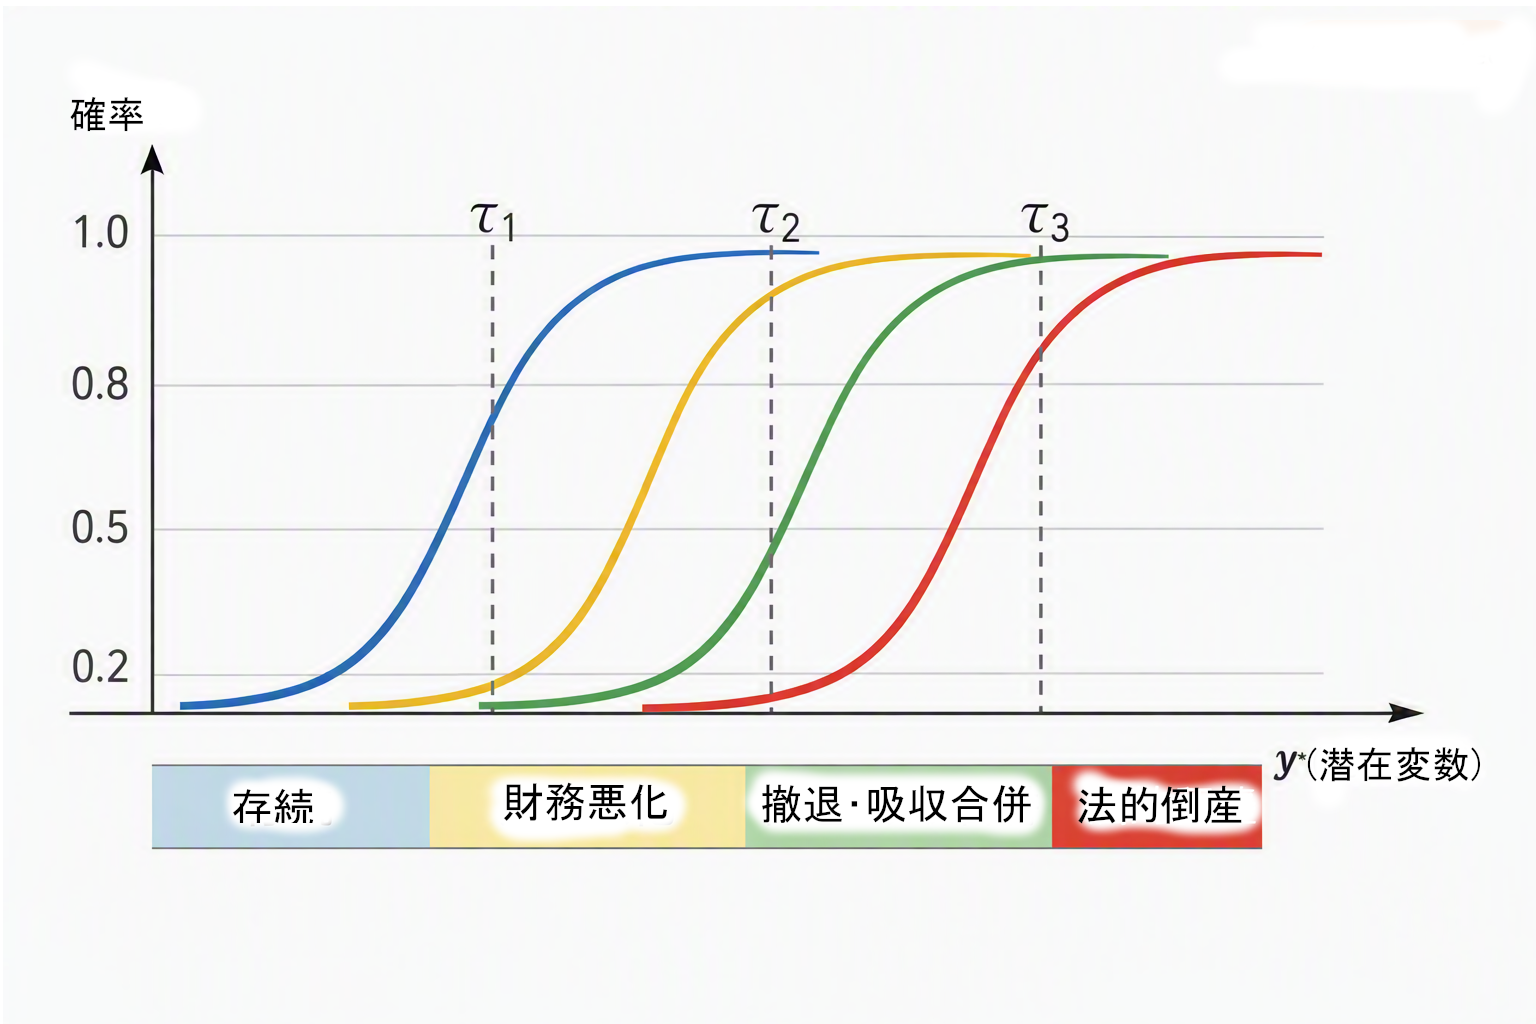
\includegraphics[width=0.85\textwidth]{figures/fig_thresholds.png}
  \caption{Ordered Logit モデルにおける閾値構造と倒産段階の概念図}
  \label{fig:thresholds}
\end{figure}

本研究では倒産ステージを以下の 4 段階に定義する。

\begin{equation}
\text{default\_stage}_{i,t} =
\begin{cases}
0 & (y^*_{i,t} < \tau_1) \\
1 & (\tau_1 \le y^*_{i,t} < \tau_2) \\
2 & (\tau_2 \le y^*_{i,t} < \tau_3) \\
3 & (\tau_3 \le y^*_{i,t})
\end{cases}
\label{eq:ordered_stages}
\end{equation}

\footnote{
閾値 $\tau_k$ は研究者が任意に設定する境界ではなく，
データから推定される内生的パラメータである点が重要である。
これは，潜在変数モデルと観測データの整合性を最も高めるように，
cutpoint が自動的に調整されることを意味する。
}

% ------------------------------------------------------------
% 5.4 Ordered Logit の確率式と cutpoint の推定
% ------------------------------------------------------------

\section{Ordered Logit の確率式と cutpoint の推定}

Ordered Logit の確率式は次のように表される。

\begin{equation}
\Pr(y=k)
=
\Lambda(\tau_k - X\beta)
-
\Lambda(\tau_{k-1} - X\beta)
\label{eq:ordered_prob}
\end{equation}

この式は，潜在変数が cutpoint をどこまで超えるかによって，
各ステージの発生確率が決まることを示している。

cutpoint $\tau_k$ は外生的に設定する値ではなく，
ロジット係数 $\beta$ と同様に尤度最大化（MLE）によって推定される。

\footnote{
cutpoint が推定されるという性質は，
Ordered Logit が「潜在変数の連続スケールをどのように区切るべきか」を
データから学習するモデルであることを意味する。
これは，研究者が恣意的に境界を設定する必要がないという利点を持つ。
}

% ------------------------------------------------------------
% 5.5 Ordered Logit の推定：尤度関数と MLE
% ------------------------------------------------------------

\section{Ordered Logit の推定：尤度関数と MLE}

閾値 $\tau_k$ は，ロジット係数 $\beta$ と同様に，
尤度最大化（MLE）によって推定される。

\begin{equation}
\Pr(y=k)=\Lambda(\tau_k - X\beta)-\Lambda(\tau_{k-1}-X\beta)
\label{eq:ordered_mle}
\end{equation}

実際の推定は Python の \texttt{statsmodels} が内部で自動的に行うため，
研究者が行列計算や反復アルゴリズムを手作業で実装する必要はない。

\footnote{
MLE は，尤度関数を最大化するパラメータを探索する数値最適化手法である。
Ordered Logit のような非線形モデルでは，
勾配ベクトルやヘッセ行列を用いた反復計算が必要となるが，
統計ライブラリが内部で自動的に処理する。
}

% ------------------------------------------------------------
% 5.6 線形倒産距離 Z_lin と潜在変数 y* の構造的対応
% ------------------------------------------------------------

\section{線形倒産距離 $Z_{\text{lin}}$ と潜在変数 $y^*$ の構造的対応}

第4章で導出した線形倒産距離 $Z_{\text{lin}}$ は，

\begin{equation}
Z_{\text{lin}} = a\mu - b\sigma + cS - dThr
\label{eq:zlin_recall}
\end{equation}

という連続的な倒産距離である。

Ordered Logit の潜在変数モデルは，

\begin{equation}
y^*_{i,t}
=
\beta_1 D_{i,t}
+ \beta_2 \mu_{i,t}
+ \beta_3 \sigma_t
+ \beta_4 S_{i,t}
+ \varepsilon_{i,t}
\label{eq:latent_y}
\end{equation}

であり，構造的に $Z_{\text{lin}}$ と一致する。

図 \ref{fig:ordered_logit_stages} は，
潜在変数の値が右側へ移動するにつれて，
倒産ステージの確率がどのように入れ替わるかを示す。

\begin{figure}[H]
    \centering
    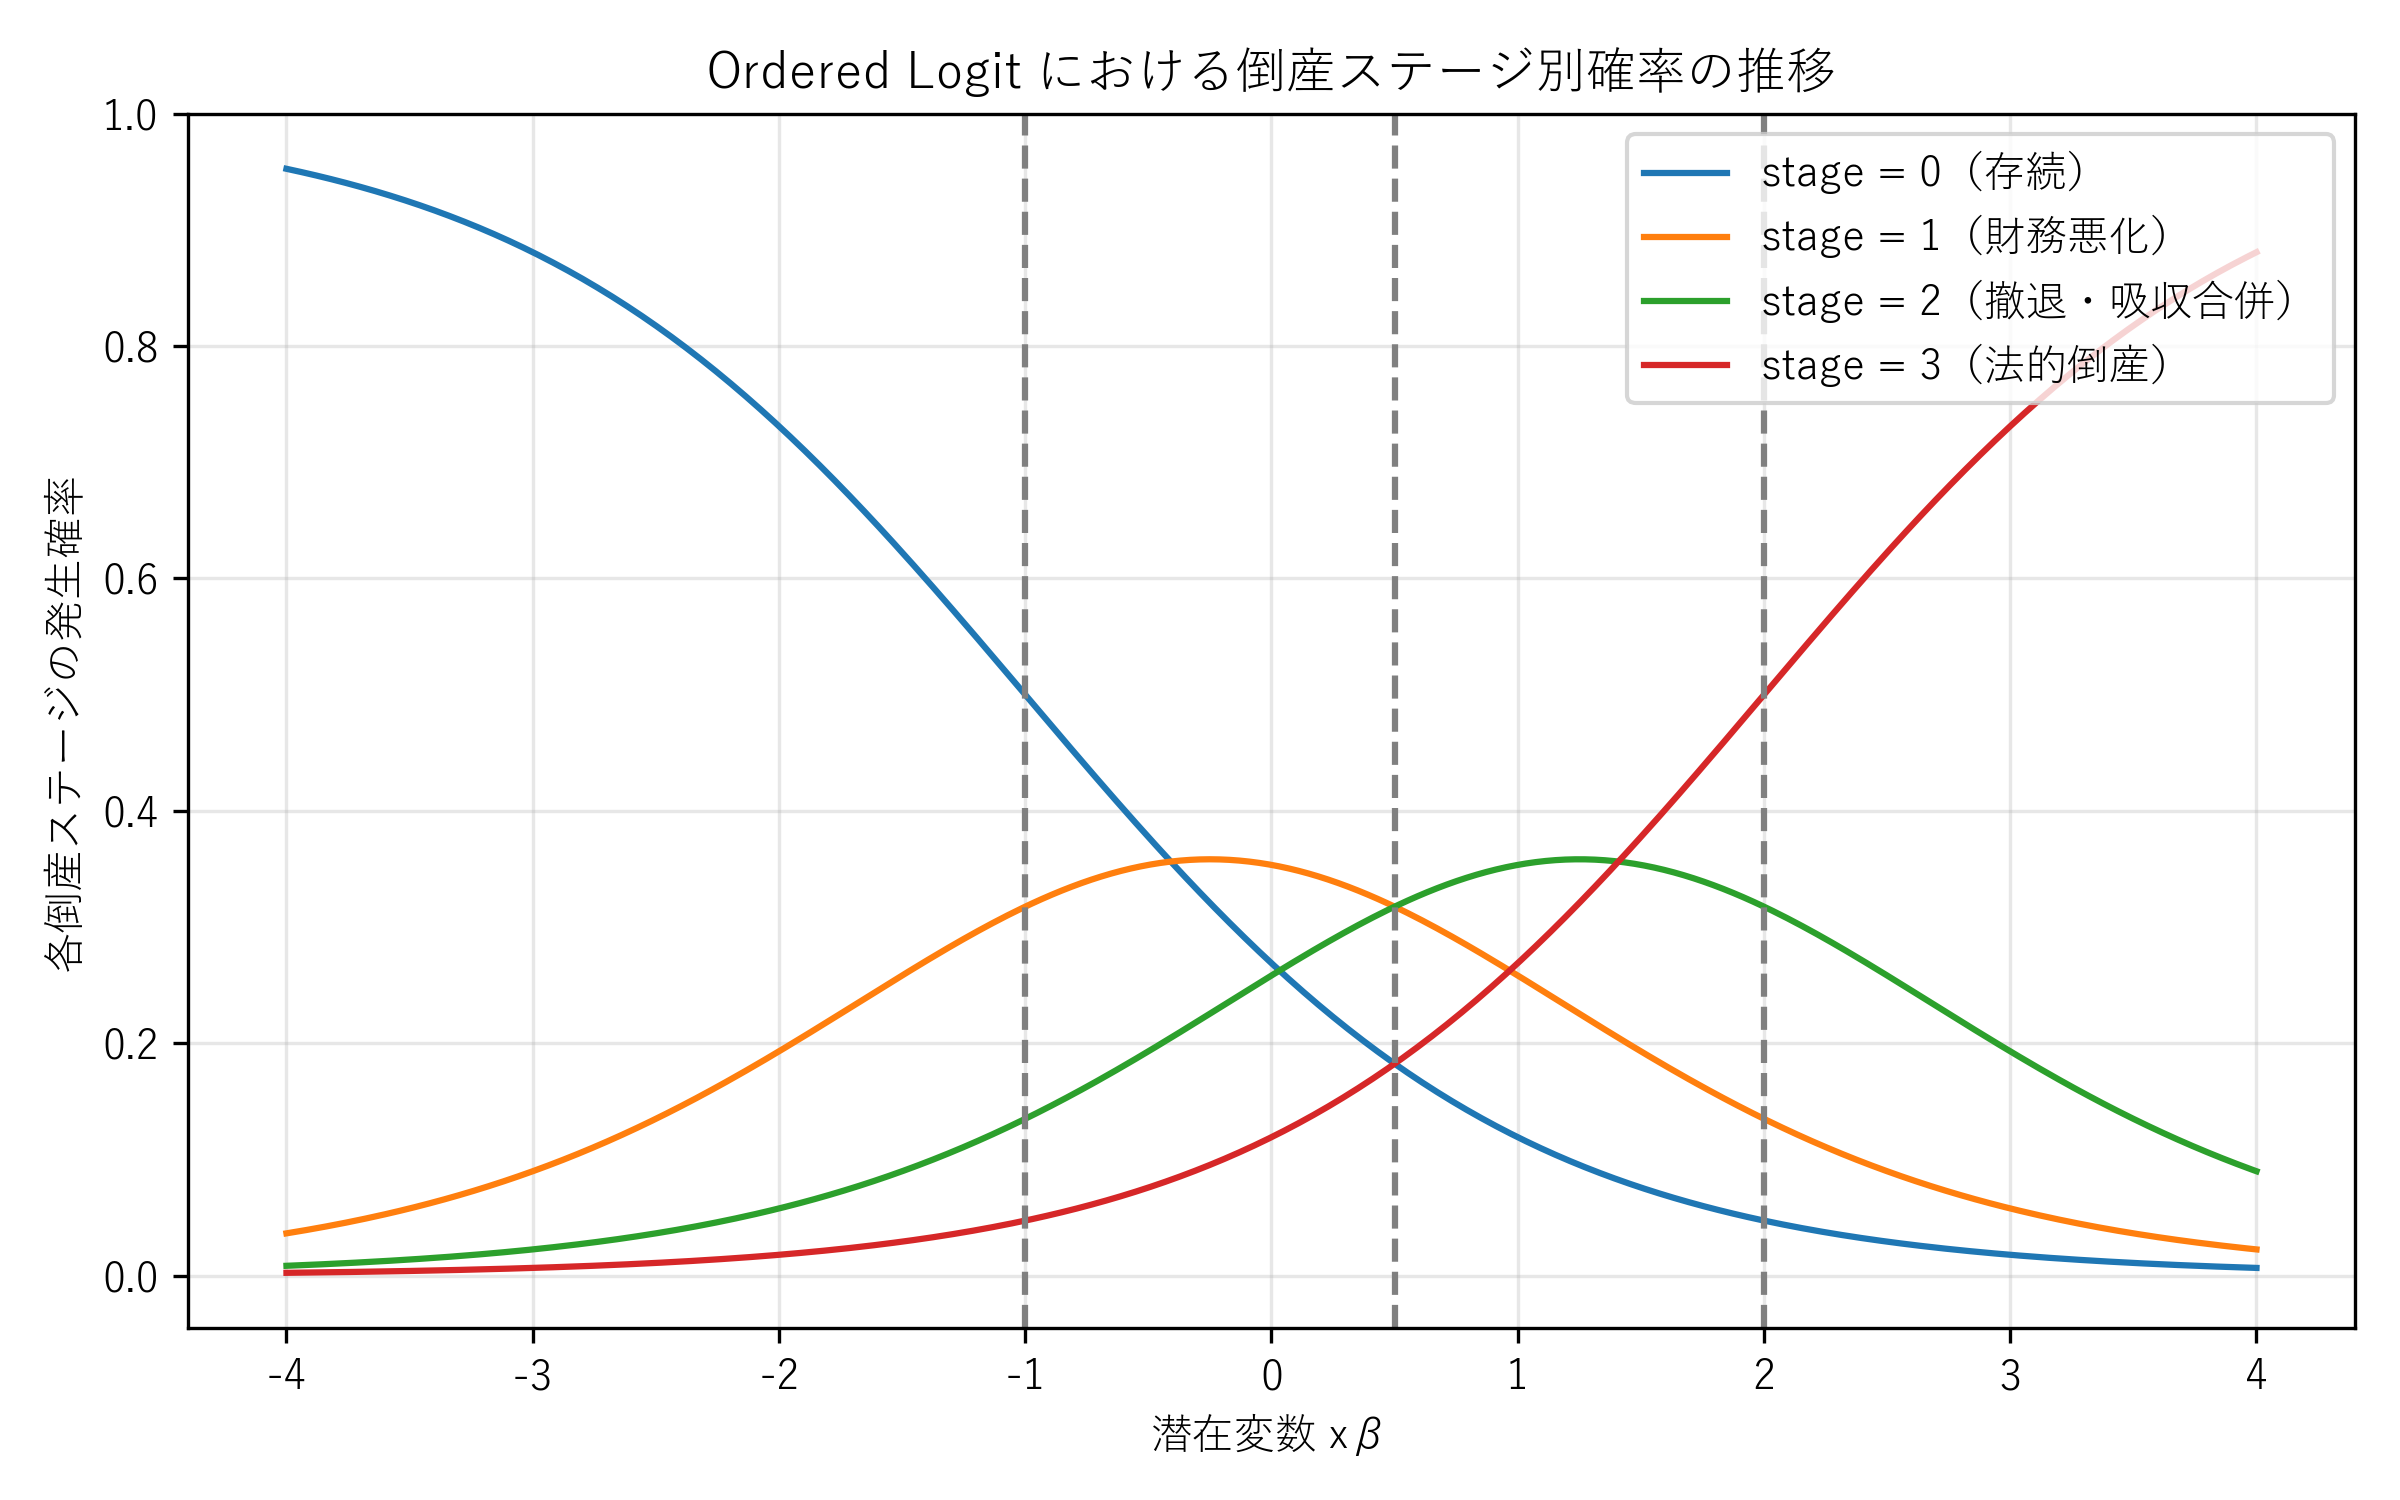
\includegraphics[width=0.85\linewidth]{figures/ordered_logit_stages.png}
    \caption{潜在変数の値と倒産ステージ確率の関係}
    \label{fig:ordered_logit_stages}
\end{figure}

\footnote{
潜在変数 $y^*$ が右側へ移動するほど，
より深刻な倒産ステージの確率が高まるという構造は，
ロジスティック曲線の性質と整合的である。
この図は，潜在変数の連続的な変化が，
離散的な倒産ステージへどのように写像されるかを直感的に理解するための補助図である。
}

% ------------------------------------------------------------
% 5.7 記号整理：潜在変数・倒産距離・閾値の対応
% ------------------------------------------------------------

\section{記号整理：潜在変数・倒産距離・閾値の対応}

\begin{table}[htbp]
\centering
\caption{潜在変数／倒産距離／閾値の記号整理}
\label{tab:latent_vars}
\begin{tabular}{lll}
\hline
記号・呼称 & 数式上の定義 & 経済的意味 \\
\hline
$y^*$ & $X\beta$ & 潜在倒産リスク（連続値） \\
$Z_{\text{lin}}$ & $X\beta$ & 線形倒産距離（倒産閾値からの距離） \\
線形予測子 & $X\beta$ & 倒産リスク要因の総合効果 \\
$\tau_k$ & cutpoints & 倒産ステージを区切る閾値 \\
$y$ & 0--3 & 観測される倒産ステージ \\
\hline
\end{tabular}
\end{table}

以上により，理論モデルの倒産距離 $Z_{\text{lin}}$ と，
実証モデルの潜在変数 $y^*$ が構造的に整合的であることが確認される。

